\chapter{Grid Search}
\label{ch4}
This chapter walks through the methodology used to select the best model and parameters to forecast 4 hours of $C_{n}^{2}$ given prior environmental measurements, then the statistical analysis performed as a justification for the model selection. Model performance is evaluated with the \ac{RMSE} between model output and truth. The \ac{RMSE} is given by
\begin{equation} \label{eq:RMSE}
	l = \sqrt{\frac{1}{N} \sum_{n=1}^{N} \left(x_{n} - y_{n}\right)^{2}}.
\end{equation}

\section{Methodology}
\label{sec:grid_search_methodology}
Given a problem to model with machine learning there are model hyperparameters to adjust in infinitely many combinations, each of which can impact model performance. Just a few examples of these hyperparameters are the optimization algorithm, the learning rate of the optimization algorithm, the number of layers in a model architecture and the number of nodes per layer. Given the many combinations of a model's hyperparameters, a careful method to determine the best combination must be employed. The definition of the ``best" model is the model which results in the best performance when applied to the validation dataset, a subset of the entire dataset specifically held from training for hyperparameter tuning. By holding back the validation dataset, an unbiased optimization of the hyperparameters can be performed. The model and parameters which performs best on the validation dataset is then applied to the test dataset for another unbiased evaluation of the final model.

There are many methods of hyperparameter optimization, but common methods are grid search and random search. Grid search, or a parameter sweep, is an exhaustive search through manually specified hyperparameters. If iterating over only one hyperparameter, for example three different learning rates, three models are trained with the three learning rates. A model is trained with the first learning rate and it's performance on the validation dataset is recorded, then another model is trained but with the second learning rate and the performance on the validation dataset is recorded. This is done once more for the third learning rate. The performance of the models with the three learning rates are compared and the best learning rate is the learning rate used by the model that performed best. This method can quickly explode in computation time as the number of hyperparameters to iterate increases. For example, iterating over two hyperparameters of three values each results in nine combinations of hyperparameters. The number of combinations is defined as the multiple of the number of values across each hyperparameter, so if there are five hyperparameters with 1, 2, 3, 4, and 5 values, then the total number of combinations is $1 \times 2 \times 3 \times 4 \times 5 = 120$ combinations.

The other common method, the random search, replaces the exhaustive grid search by randomly selecting hyperparameters within defined bounds. An algorithm randomly selects the hyperparameters and models are trained with the different combinations then applied to the validation dataset to evaluate performance. A benefit of the random search is the selection of parameter combinations that might not be defined in a grid search.

In this work the grid search is employed because prior knowledge of hyperparameters is unknown, thus the exhaustive grid search is necessary to explore a wide range of combinations. This grid search iterates over five parameters. The outermost parameter is the four fundamental architectures: \ac{MLP}, simple \ac{RNN}, \ac{GRU-RNN}, and \ac{LSTM-RNN}. The \ac{MLP} is a common machine learning architecture and serves as a baseline. The simple \ac{RNN}, \ac{GRU-RNN}, and \ac{LSTM-RNN} are variants of the general \ac{RNN} and are searched to find if a specific variant is better or worse than the others when applied to this problem. The next parameter is the input sequence variables used by the model. From Section \ref{sec:wx_seq_hist}, the available input sequence features (variables) are prior temperature, pressure, relative humidity, wind speed, solar irradiance, and $C_{n}^{2}$ measurements. The \textit{input features} parameter iterates over which features (variables) to train the model. Since there are six available features, and each feature can only be used or not used, there are $2^6 = 64$ total combinations. However, a threshold is set to train on a minimum of four features which reduces the total number of input feature combinations to 22. This threshold is set to discourage the model from memorizing one or two features, and for a significant reduction in computation time.

The third search parameter is the \textit{input sequence length}. Independent of the input features (variables), in a single sequence/forecast the amount of information available to the model is dependent on the time-length of the input sequence. Whether the model performs best with only 4 hours of input data or 16 hours of input data is highly relevant information. Thus, four lengths of the input sequence are searched: 4, 8, 12, and 16 hours. These lengths are chosen to be $1\times$, $2\times$, $3\times$, and $4\times$ the 4 hour forecast length. Note that the train, validation, and test datasets are carefully formatted so the same forecasts are trained, validated, and tested regardless of the input sequence length. This avoids an instance where a 4 hour input sequence might exist for a particular forecast but a 16 hour input sequence is not available due to missing data. The fourth parameter searched is the number of hidden layers in each architecture: 1 or 2. The fifth and final searched parameter is the number of hidden nodes per hidden layer: 10 through 50 in steps of 10. The final two parameters essentially search over the number of parameters in the model with some variation in the interaction of those parameters. Each fundamental architecture in total iterates over $22 \times 4 \times 2 \times 5 = 880$ combinations of parameters. Due to the stochastic nature of model training, a single model could perform significantly different than another model trained with the same parameters, thus a total of 10 models are trained per combination per fundamental architecture to ensure the stability of results. In this search a total of $880 \times 4 \times 10 = 35,200$ models are trained.

For each model trained in the grid search the following parameters are fixed: mini-batch size, optimization algorithm, initial learning rate, learning rate decay (step and decay factor), and weight decay. The mini-batch size, the number of training examples used per model parameter update, is set to 32 yielding a total of 30 parameter updates (933/32) per epoch (iteration through the entire dataset). The optimization algorithm is AdamW\cite{kingma2017adam} \cite{loshchilov2019decoupled}. The initial learning rate is 0.01 and decays by a factor of 10 every 10 epochs. This results in learning rates 0.01, 0.001, 1e-4, 1e-5, and 1e-6 from epochs 1 - 10, 11 - 20, 21 - 30, 31 - 40, and 41 - 50, respectively. The high initial learning rate is to ensure suitably-high gradients are back-propagated through the model to allow each model 10 epochs (300 total parameter updates) to escape any local minima. This training method consistently leads to a strong model convergence in only a few seconds. The weight decay is a regularization technique applied to the optimization algorithm and is 0.001.

\section{Grid Search Results}
The analyses of the grid search are performed independently on each architecture. From the four grid searches, four 2d-arrays of \ac{RMSE} loss scores, the performance metric between validation truth and output $log_{10}(C_{n}^{2})$, are recorded for analysis. The 2d-arrays are shape $880 \times 10$ for 880 parameter combinations and 10 models each. From these four 2d arrays, the average and standard deviation of the \ac{RMSE} scores are calculated per parameter combination yielding four arrays of 880 averages and standard deviations. The standard deviation, the square root of the average of the squared deviations from the mean, is calculated by
\begin{equation} \label{eq:standard_deviation}
	\sigma = \sqrt{\frac{\sum\left(x - \bar{x}\right)^{2}}{N - ddof}}
\end{equation}
where $\sigma$ is the standard deviation, $x$ is the data, $\bar{x}$ is the average of the data, N is the number of data points, and $ddof$ is the delta degrees of freedom. Using $ddof = 1$ provides an unbiased estimator of the variance of the infinite population. It is standard practice to use $ddof = 1$. $ddof = 0$ should be used in the situation of measuring the variance of a distaribution whose mean $\bar{x}$ is known a priori rather than being estimated from the data \cite{10.5555/1403886}.

If the average, $\bar{x}$ in Equation \ref{eq:standard_deviation}, were calculated many times with different sets of sampled data the values of $\bar{x}$ would themselves have a standard deviation. This is called the \textit{standard error} of the estimated mean $\bar{x}$. Assuming the underlying distribution is Gaussian, the \textit{standard error} is given approximately by
\begin{equation} \label{eq:standard_error}
	\sigma_{\bar{x}} = \frac{\sigma}{\sqrt{N}},
\end{equation}
where $\sigma_{\bar{x}}$ is the standard error of the mean, $\sigma$ is the standard deviation from Equation \ref{eq:standard_deviation}, and $N$ is the number of samples used the calculate $\bar{x}$ \cite{10.5555/1403886}. In the calculation of the standard error of the average loss scores, $N$ is 10, the number of models trained for each combination of the grid search. From these statistics the best model as applied to the validation dataset is determined and significance quantified.

\subsection{Results Sorting}
The four arrays of average RMSE scores are sorted from best to worst and the sort indices are applied to the array of grid search parameters. From these sorted arrays the best model and its parameters are extracted. Figure \ref{fig:grid_search_results} illustrates the validation average $log_{10}(C_{n}^{2})$ RMSE loss as a function of the sorted index. Figure \ref{fig:grid_search_results_a} plots all 880 sorted scores for each fundamental architecture. Figure \ref{fig:grid_search_results_b} plots only the first ten to focus on the best performers. In each plot \ac{MLP} is drawn in blue, simple \ac{RNN} in orange, \ac{GRU-RNN} in green, and \ac{LSTM-RNN} in red. The curves in each figure are monotonically increasing because the sorted losses are plotted. Figure \ref{fig:grid_search_results_b} additionally plots the standard error.
\begin{figure}[h!]
	\centering
	\subfloat[Full set of iterations\label{fig:grid_search_results_a}]{
		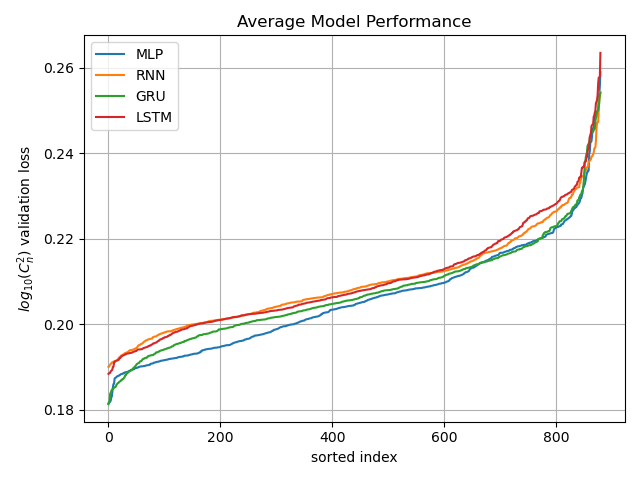
\includegraphics[width=0.49\textwidth]{average_model_performance_wide.png}
	}
	\subfloat[Top 10 iterations\label{fig:grid_search_results_b}]{
		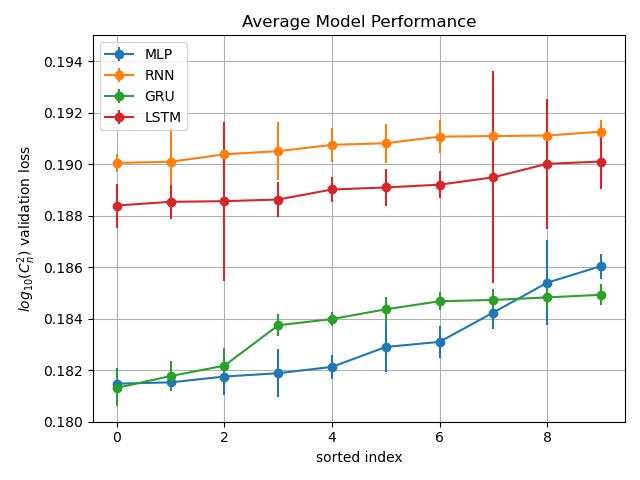
\includegraphics[width=0.49\textwidth]{average_model_performance_narrow.png}
	}
	\hfill
	\caption{Grid search results.}
	\label{fig:grid_search_results}
\end{figure}
The general shape of the sorted loss curves are highly correlated from architecture to architecture and their slopes are consistent from sorted index 100 through 800. On either side, between sorted indices 0 through 100, and 800 through 880, the curves exponentially increase. This is an indication that there are a general set of modeling parameters which are notably better than all the others, and likewise a set that are far worse than the others.

In terms of model performance, the curves in Figure \ref{fig:grid_search_results_a} generally indicate that over the grid search space the \ac{MLP} dominates the ensemble of \ac{RNN} architectures. Throughout the sorted indices, but most importantly at the beginning (left) of the sorted indices, the \ac{MLP} (blue) and \ac{GRU-RNN} (green) architectures perform better by a large margin compared with the simple \ac{RNN} (orange) and \ac{LSTM-RNN} (red) architectures. This is further shown in Figure \ref{fig:grid_search_results_b} which illustrates the first ten sorted indices of Figure \ref{fig:grid_search_results_a}. The loss curves illustrate that on average the best ten models of the simple \ac{RNN} is the worst of the four architectures and the best ten models of the \ac{LSTM-RNN} models are a small scale factor better. This result is interesting since the \ac{MLP} is the baseline architecture and the ensemble of \ac{RNN}s are designed to handle time series data. Another notable feature of the top ten \ac{LSTM-RNN} models in Figure \ref{fig:grid_search_results_b} is the large standard error of the mean calculated from Equation \ref{eq:standard_error}. This is an indication of significant variance in performance over the 10 models trained per grid search iteration. During brief analysis two \ac{LSTM-RNN} models trained on the same parameters could illustrate impressive then poor performance. This high variability is not desirable and leads to high average RMSE, but does reveal the capability of the \ac{LSTM-RNN} if the right set of training parameters can consistently result in a good model.

Further evaluation of the loss curves in Figure \ref{fig:grid_search_results_b} shows that the best ten \ac{MLP} and \ac{GRU-RNN} models are very similar, even crossing each other twice. Of the top ten \ac{MLP} and \ac{GRU-RNN} models, the very best of each (sorted index 0) show that the \ac{GRU-RNN} is slightly better with a validation average $log_{10}(C_{n}^{2})$ of 0.181316 vs. 0.181476 for the \ac{MLP}. The standard errors are also very similar, 0.000697 vs. 0.000605, for the \ac{GRU-RNN} and \ac{MLP}, respectively. Thus the consistency of model convergence for one model is not notably better than the other. Generally the standard error bars of the \ac{MLP} and \ac{GRU-RNN} architectures in Figure \ref{fig:grid_search_results_b} are smaller (better) than the bars of the simple \ac{RNN} and especially the \ac{LSTM-RNN} architectures. These results illustrate that of the four architectures, the \ac{MLP} and \ac{GRU-RNN} are proving to be best suited for this problem as evaluated on the validation dataset.

\subsection{Statistical Significance}
The results presented in Figure \ref{fig:grid_search_results} clearly show that specific architectures and corresponding parameters perform better on the validation dataset than others. However, from the top performing models there is little discrepancy in performance metric which introduces ambiguity into which model and parameter combination is the very best. To sort through these similar models is the \textit{Student's t-test} which is a test of whether two sample means are different to a specific level of significance. Performing tests of significance on the results in Figure \ref{fig:grid_search_results_b} statistically distinguishes the models to show if a model is significantly better than another.

\subsubsection{\textit{Student's t-test} Foundation}
\label{sec:students_t-test}
The \textit{Student's t-test} is a statistical test of the null hypothesis $H_{0}$ that two samples have equal means. The alternative hypothesis $H_{a}$ is that samples do not have equal means. The foundation of the test is as follows. Take one set of measurements, then some event happens, then take another set of measurements. Did the event, like a change in a control parameter, make a difference? In this work the measurements are model performances on the validation dataset and the event is a change in the model parameters. There are several variations of the \textit{Student's t-test} including the \textit{independent t-test} for equal and unequal variances, and the \textit{dependent t-test} for paired samples. The \textit{independent t-test} for unequal variances is used in this work because the samples are independent and the variances are not assumed to be equal. This specific test is known as \textit{Welch's t-test} and given samples $x_{A}$ and $x_{B}$ defines the statistic \textit{t} as
\begin{equation} \label{eq:t_stat}
	t = \frac{\bar{x_{A}} - \bar{x_{B}}}{\sqrt{\frac{Var(x_{A})}{N_{A}} + \frac{Var(x_{B})}{N_{B}}}},
\end{equation}
where $\bar{x_{A}}$, $Var(x_{A})$ and $N_{A}$ are the sample A mean, variance and size, respectively. Likewise, $\bar{x_{B}}$, $Var(x_{B})$ and $N_{B}$ are the sample B mean, variance and size. The two-tailed $p$-value or significance of this value of \textit{t} is calculated with $dof$ degrees of freedom
\begin{equation} \label{eq:t_dof}
	dof = \frac{\left[\frac{Var(x_{A})}{N_{A}} + \frac{Var(x_{B})}{N_{B}}\right]^{2}}{\frac{\left[Var(x_{A})/N_{A}\right]^{2}}{N_{A} - 1} + \frac{\left[Var(x_{B})/N_{B}\right]^{2}}{N_{B} - 1}}.
\end{equation}
The $p$-value is a number between zero and one and is the probability that $|t|$ (hence two-tailed) could be this large or larger just by chance under the assumption that the null hypothesis $H_{0}$ is correct \cite{10.5555/1403886}. A very small p-value ($\le$ 0.05) means that the observed difference in means is very significant and the null hypothesis $H_{0}$ is rejected at the 5\% significance level. This does not, however, prove that the null hypothesis $H_{0}$ is false or the alternative hypothesis $H_{a}$ is true. A low $p$-value means \textit{either} that the null hypothesis is true and a highly improbable event has occurred \textit{or} that the null hypothesis is false.

\subsubsection{\textit{Student's t-test} Results}
The \textit{Student's t-test} described in above is robustly implemented as a function from \textit{SciPy}, a Python-based open-source software for mathematics, science, engineering, and most importantly in this case, statistics \cite{2020SciPy-NMeth}. Using the $ttest\_ind$ function and setting parameter $equal\_var$ to False performs the \textit{Welch's t-test} given two arrays of measurements.

The \textit{t-test} is performed on each of the top ten models in Figure \ref{fig:grid_search_results_b} where sample A in Equations \ref{eq:t_stat} and \ref{eq:t_dof} is the 10 validation $log_{10}(C_{n}^{2})$ RMSE scores from the very best \ac{GRU-RNN} model. Sample B in Equations \ref{eq:t_stat} and \ref{eq:t_dof} iterates through the 10 validation RMSE scores of the rest of the models in Figure \ref{fig:grid_search_results_b}. This results in $p$-values of the best \ac{GRU-RNN} model evaluated against the next nine best \ac{GRU-RNN} models and the best ten \ac{MLP} models, simple \ac{RNN} models, and \ac{LSTM-RNN} models. A significance level ($\alpha$) of 0.05 is predefined to reject the null hypotheses $H_{0}$ if the $p-$value is $\le \alpha$. Figure \ref{fig:students_t-test} summarizes these results by plotting the two-tailed $p$-value as a function of the sorted index, the same x-axis as in Figure \ref{fig:grid_search_results_b}. The $p$-values are again parsed by fundamental architecture.
\begin{figure}[h!]
	\centering
	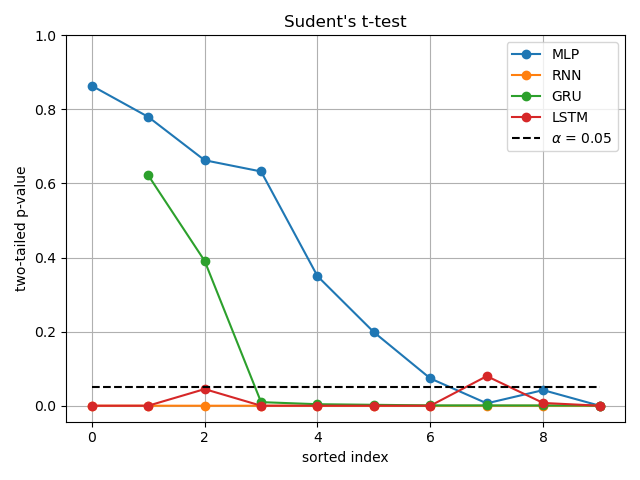
\includegraphics[width=0.7\textwidth]
	{students_t-test.png}
	\hfill
	\caption{\textit{Welch's t-test} of the grid search results}
	\label{fig:students_t-test}
\end{figure}
The \ac{MLP} $p$-values are in blue, simple \ac{RNN} in orange, \ac{GRU-RNN} in green, and \ac{LSTM-RNN} in red. The black dashed line in Figure \ref{fig:students_t-test} is the $p$-value threshold $\alpha = 0.05$. The \ac{GRU-RNN} $p$-value at sorted index 0 (zero) is omitted because performing the \textit{Welch's t-test} on the best \ac{GRU-RNN} model against itself is irrelevant.

Any markers below the black dashed line ($\alpha$) in Figure \ref{fig:students_t-test} represent models whose mean performance is statistically different from the best \ac{GRU-RNN} model at the 5\% level, a rejection of the null hypothesis $H_{0}$. Since the best \ac{GRU-RNN} model is the best performing model in the entire grid search, the models below the $\alpha$ line are statistically worse at the 5\% level. Any markers above the $\alpha$ line represent models whose performance is not statistically worse, i.e., the null hypothesis $H_{0}$ is not rejected at the 5\% level. A total of ten markers in Figure \ref{fig:students_t-test} are above the $\alpha$ line: two are the next two best \ac{GRU-RNN} models, seven are the seven best \ac{MLP} models, and one is the eighth best \ac{LSTM-RNN} model. The \ac{LSTM-RNN} model which does not reject the null hypothesis is a result of the high variance in the model illustrated by the large standard error bars in Figure \ref{fig:grid_search_results_b} at sorted index 8 on the x-axis. Likewise, the standard error bars at sorted index 3 in Figure \ref{fig:grid_search_results_b} also correspond with the $p$-value that is nearly to the $\alpha$ line in Figure \ref{fig:students_t-test}.

The other markers above the $\alpha$ line from \ac{MLP} and \ac{GRU-RNN} are consistent with the average RMSE scores in Figure \ref{fig:grid_search_results_b}. The first three \ac{GRU-RNN} scores in Figure \ref{fig:grid_search_results_b} hover around 0.182 with the first three \ac{MLP} scores. Then the \ac{GRU-RNN} scores step up to nearly 0.184 and steadily increase. The \ac{MLP} scores steadily rise until the seventh sorted index where there is a notable step above 0.184. The indices of these steps, three for \ac{GRU-RNN} and seven for \ac{MLP}, also are the first models where the null hypothesis is rejected at the 5\% level. This is illustrated in Figure \ref{fig:students_t-test} by the \ac{GRU-RNN} (green) marker at sorted index 3 being the first \ac{GRU-RNN} model below the $\alpha$ line and the \ac{MLP} marker at sorted index 7 being the first \ac{MLP} model below the $\alpha$ line.

\section{Evaluation of Best Models}
\subsection{Comparative Analysis}
From the results in Figure \ref{fig:students_t-test}, the top three \ac{GRU-RNN} models and top seven \ac{MLP} models are selected for further evaluation because they fail to reject the \textit{Welch's t-test} null hypothesis. The \ac{LSTM-RNN} model which also does not reject the null hypothesis is not considered for further evaluation because its rejection is explained by the very high standard error. Mentioned above, the indices to sort the validation average $log_{10}(C_{n}^{2})$ RMSE scores are used to sort the corresponding grid search parameters. Table \ref{tab:grid_search_results_GRU} summarizes the grid search parameters associated with the top three \ac{GRU-RNN} models.
\begin{table}[h!]
	\begin{center}
		\caption{Top GRU-RNN Model Parameters}
		\label{tab:grid_search_results_GRU}
		\begin{tabular}{||l|c|c|c|c||}
			\hline
			Model & Sequence Features & Sequence Length (hours) & Layers & Nodes \\
			\hline
			\hline
			GRU-RNN 1 & Press, RH, SI, $C_{n}^{2}$ & 12 & 2 & 40 \\
			\hline
			GRU-RNN 2 & Press, RH, SI, $C_{n}^{2}$ & 12 & 2 & 50 \\
			\hline
			GRU-RNN 3 & Press, RH, SI, $C_{n}^{2}$ & 12 & 2 & 30 \\
			\hline
		\end{tabular}
	\end{center}
\end{table}
The three rows in Table \ref{tab:grid_search_results_GRU} (ignoring the header) represent the best \ac{GRU-RNN} model (\ac{GRU-RNN} 1), then the next two best \ac{GRU-RNN} models (\ac{GRU-RNN} 2 and \ac{GRU-RNN} 3). The columns in Table \ref{tab:grid_search_results_GRU} sort the grid search parameters into ``Sequence Features" which is the input sequence features (variables) used by the model, ``Sequence Length (hours)" that is the length of input sequence data used by the model and is reported in number of hours, ``Layers" which is the number of layers used by each model, and ``Nodes" which is the number of nodes per layer in each model.

The summary in Table \ref{tab:grid_search_results_GRU} is remarkably consistent. The input sequence features used by all three of the best models are pressure, relative humidity, solar irradiance and $C_{n}^{2}$, the sequence length of each model is 12 hours, the number of \ac{GRU-RNN} layers for each model is two, and the number of nodes per \ac{GRU-RNN} layer is 40, 50, and 30 in order of the top three \ac{GRU-RNN} models. The consistency of the parameters from model-to-model indicates a specific type of model has been found to best perform on the validation dataset. It is also encouraging that the best \ac{GRU-RNN} model uses 40 nodes per layer, then 50, and finally 30. If the best \ac{GRU-RNN} used 50 nodes, for example, a concern would arise of whether the bounds of the grid search were wide enough, i.e., the number of nodes covered in the grid search have gone higher than 50.

Similarly to Table \ref{tab:grid_search_results_GRU}, Table \ref{tab:grid_search_results_MLP} summarizes the grid search parameters for the top seven \ac{MLP} models.
\begin{table}[h!]
	\begin{center}
		\caption{Top MLP Model Parameters}
		\label{tab:grid_search_results_MLP}
		\begin{tabular}{||l|c|c|c|c||}
			\hline
			Model & Sequence Features & Sequence Length (hours) & Layers & Nodes \\
			\hline
			\hline
			MLP 1 & Temp, Press, RH, SI & 16 & 2 & 30 \\
			\hline
			MLP 2 & Temp, Press, RH, SI & 16 & 2 & 40 \\
			\hline
			MLP 3 & Temp, Press, RH, SI & 16 & 2 & 50 \\
			\hline
			MLP 4 & Temp, Press, RH, SI & 16 & 2 & 20 \\
			\hline
			MLP 5 & Temp, Press, RH, SI & 12 & 2 & 40 \\
			\hline
			MLP 6 & Temp, Press, RH, SI & 12 & 2 & 30 \\
			\hline
			MLP 7 & Temp, Press, RH, SI & 12 & 2 & 50 \\
			\hline
		\end{tabular}
	\end{center}
\end{table}
Evaluation of Table \ref{tab:grid_search_results_MLP} again yields consistency of the best \ac{MLP} models. For each of the models the input sequence features are temperature, pressure, relative humidity, and solar irradiance. The input sequence length is 16 hours for the first four models, then 12 hours for the last three. The number of hidden \ac{MLP} layers is two for all seven models. Finally, the number of nodes is 30, 40, 50, then 20 for the 16 hour sequence lengths (first four models), then 40, 30, and 50 for the 12 hour sequence lengths (last three models).

The consistency of input sequence features in the best \ac{MLP} models is encouraging because like the best \ac{GRU-RNN} models, a specific type of \ac{MLP} model has been found to perform best on the validation dataset. It's also encouraging that the number of hidden layers in the \ac{MLP} model is consistently 2 across all seven models. The ordering of the sequence lengths and number of nodes per hidden layer in Table \ref{tab:grid_search_results_MLP} illustrates that using 16 hours of input sequences and at least 20 nodes per layer is better than using 12 hours of input sequences and at least 30 nodes per layer. Most importantly, though, is shows that that using 12 hours of input sequences and at least 30 nodes is better than 16 hours of input sequences with only 10 nodes. This is an indication that using only 10 nodes per layer in the \ac{MLP} likely does not yield the model complexity to perform well on the validation dataset.

There are two major distinctions between the best \ac{GRU-RNN} and \ac{MLP} models summarized in Tables \ref{tab:grid_search_results_GRU} and \ref{tab:grid_search_results_MLP}. First, the input sequences each only use four features (variables), but the features used by each architecture are different. Both architectures use pressure, relative humidity, and solar irradiance, but the \ac{GRU-RNN} architecture uses $C_{n}^{2}$ and \ac{MLP} uses temperature. It's interesting that the use of temperature, one of the most fundamental weather variables and oscillatory in character, is not used by the best \ac{GRU-RNN} models. It's more interesting, however, that the best \ac{MLP} models do not use prior $C_{n}^{2}$ measurements as an input. It's expected that the prior $C_{n}^{2}$ measurements would be a significant driver of the model outputs since generally the trend of recent measurements would continue in the future, so it's curious that the best \ac{MLP} models deviate from this expectation. The second major distinction is the input sequence lengths. The best \ac{GRU-RNN} models only require 12 hours of inputs, whereas the four best \ac{MLP} models require 16 hours of inputs. From a practical perspective, requiring four less hours of input sequences is highly desirable in a real-world application.

In addition to the different input features used by the best \ac{GRU-RNN} and \ac{MLP} models, another curious result is that only four input features are used by each architecture when up to six variables are available. To investigate further, the ``Sequence Features" column in Tables \ref{tab:grid_search_results_GRU} and \ref{tab:grid_search_results_MLP} are expanded to evaluate more models, the best 88 (10\%) and worst 88 (10\%). The simple \ac{RNN} and \ac{LSTM-RNN} are also included in this analysis. The number of times each input feature (variable) is used by the best 88 and worst 88 models is recorded per architecture. Figure \ref{fig:variable_sets_analysis} illustrates bar charts of these results.
\begin{figure}[h!]
	\centering
	\subfloat[Best 10\%\label{fig:variable_sets_analysis_a}]{
		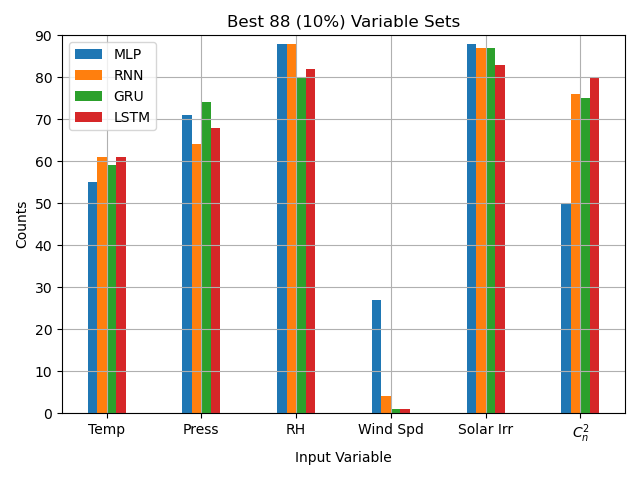
\includegraphics[width=0.49\textwidth]{bar_variable_sets_best.png}
	}
	\subfloat[Worst 10\%\label{fig:variable_sets_analysis_b}]{
		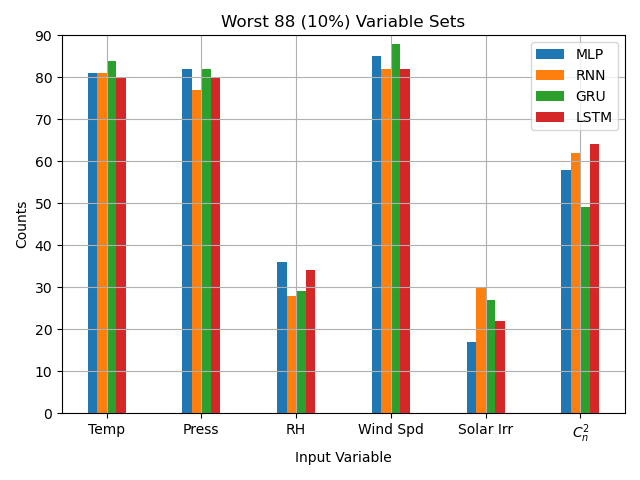
\includegraphics[width=0.49\textwidth]{bar_variable_sets_worst.png}
	}
	\hfill
	\caption{Best 10\% and worst 10\% variable sets.}
	\label{fig:variable_sets_analysis}
\end{figure}
Each category on the x-axis is an input feature, and the y-axis is the number of counts. There are four bars for each category representing the fundamental architectures. The blue bars are \ac{MLP}, orange bars are simple \ac{RNN}, green bars are \ac{GRU-RNN}, and red bars are \ac{LSTM-RNN}. Figure \ref{fig:variable_sets_analysis_a} is the counts of each input feature for the best 88 models of each architecture, and Figure \ref{fig:variable_sets_analysis_b} is the counts for the worst 88 models of each architecture.

Evaluation of best 88 models of each architecture in Figure \ref{fig:variable_sets_analysis_a} illustrates several interesting results, but one stands out in particular: wind speed is rarely used as an input feature in the best 10\% of models. Specifically, the ensemble of \ac{RNN} architectures almost never use wind speed: the simple \ac{RNN} uses wind speed four times, and the \ac{GRU-RNN} and \ac{LSTM-RNN} models only use wind speed once each. The best 88 \ac{MLP} models, however, use wind speed just under 30 times. Concurrent evaluation of the worst 88 models of each architecture in Figure \ref{fig:variable_sets_analysis_b} further reveals information about wind speed: all four fundamental architectures use wind speed in nearly all of the worst 88 models. The ensemble of \ac{RNN}s almost universally ignoring wind speed in the best models, combined with the almost universal inclusion in the worst models, is strong evidence that the exclusion of wind speed as an input feature for the best \ac{GRU-RNN} and \ac{MLP} models is not by chance. Rather, this is conclusive insight that prior wind speeds are not beneficial to the forecasting of $C_{n}^{2}$ in this problem. It is likely that this is due to the large spatial gap between the weather station and $C_{n}^{2}$ path. 

For the \ac{MLP}, the wind speed counts in Figures \ref{fig:variable_sets_analysis_a} and \ref{fig:variable_sets_analysis_b} offer some insight into how the \ac{MLP} is learning compared with the ensemble of \ac{RNN} architectures. The processing of the \ac{RNN}s essentially forces the model to learn the input sequences as a function of time, whereas the \ac{MLP}, which uses the same information in a flattened layer, is free to learn any relationships. Specifically the \ac{MLP} is not bounded to learn the temporal relationship between the input variables, thus is is reasonable to theorize that the \ac{MLP} is more prone to learning relationships that are not as physical.

Two more categories of input features stand out in Figures \ref{fig:variable_sets_analysis_a} and \ref{fig:variable_sets_analysis_b}: relative humidity and solar irradiance are nearly universally used in the best 88 models of each architecture, and are seldom used in the worst 88 models of each architecture. This result reveals the opposite conclusion about wind speed: relative humidity and solar irradiance are strong drivers of $C_{n}^{2}$ and the spatial separation between weather measurements and $C_{n}^{2}$ path does not significantly impact the models' performances, i.e., these two variables are reliably transferred across space.

Temperature and pressure in Figures \ref{fig:variable_sets_analysis_a} and \ref{fig:variable_sets_analysis_b} are two input features whose counts require careful evaluation. In the best 88 models, temperature has an average around 57 - 58 counts across the four architectures, but has 80+ counts for each architecture in the worst 88 models. Similarly, pressure has around 68-69 counts on average in the best 88 models, and around 80 counts on average in the worst 88 models. The counts in the best 88 models suggest that pressure is not as sensitive to the problem as relative humidity and solar irradiance, and temperature is even less sensitive. The counts in the worst 88 models initially suggest that temperature and pressure are generally poor input features, but the very low counts of relative humidity and solar irradiance influence that conclusion, possibly incorrectly. Because a minimum of four input variables are required by the grid search's bounds, the low counts for relative humidity and solar irradiance already account for the maximum two dropped variables, which means that temperature and pressure by default will often get used as an input to the worst 88 models. This argument is not valid for wind speed because the counts are extremely low in the best 88 models \emph{and} the counts are extremely high in the worst 88 models. As a final note about temperature and pressure, if the minimum number of input features was set to three instead of four it's possible they would be entirely excluded from the best \ac{GRU-RNN} models based on the counts in Figure \ref{fig:variable_sets_analysis_a}, leaving only relative humidity, solar irradiance, and $C_{n}^{2}$. 

The final input feature of discussion in Figures \ref{fig:variable_sets_analysis_a} and \ref{fig:variable_sets_analysis_b} is $C_{n}^{2}$. This is another input feature (wind speed) in which there is a strong difference between \ac{MLP} and the ensemble of \ac{RNN} architectures. For the best 88 models, $C_{n}^{2}$ is utilized 75+ times by the ensemble of \ac{RNN} architectures, but only 50 times by the \ac{MLP}. Most importantly, though, is that \emph{none} of the best seven \ac{MLP} architectures from Table \ref{tab:grid_search_results_MLP} use $C_{n}^{2}$. This is further evidence of the fundamental difference between the processing of the ensemble of \ac{RNN}s and the \ac{MLP}. It's expected that prior $C_{n}^{2}$ measurements is a strong driver of future $C_{n}^{2}$ and the ensemble of \ac{RNN}s strongly learn this relationship. The \ac{MLP} has not learned this relationship as strongly possibly because $C_{n}^{2}$ is only relevant to forecasting $C_{n}^{2}$ if it is processed temporally.

The counts in Figures \ref{fig:variable_sets_analysis_a} and \ref{fig:variable_sets_analysis_b} have been shown to behave as a top-level input sensitivity analysis. Many useful conclusions have been derived about how the architectures use the inputs. Further evaluation would require a significant level of time-series analysis which is beyond the scope of this effort.

\subsection{Selection of the Best Model}
The results presented in this Chapter have shown the best performing model as applied to the validation dataset. By \textit{Welch's t-test} it has been shown to be significantly better than all but nine other models at the 5\% level. The best model (\ac{GRU-RNN}) has been evaluated against the next two best \ac{GRU-RNN} models to show strong consistency in the model parameters. This same evaluation and result has been shown for the seven \ac{MLP} models. The next step in this work applies a model to the test dataset so a single model is chosen. This single model is ``GRU-RNN 1" in Table \ref{tab:grid_search_results_GRU}. It has two \ac{GRU-RNN} layers with 40 nodes each and uses 12 hours of pressure, relative humidity, solar irradiance, and $C_{n}^{2}$ as input features. This model is chosen for many reasons.
\begin{enumerate}
	\item It results in the lowest average RMSE as applied to the validation dataset.
	\item The next two best \ac{GRU-RNN} models, which are not significantly different in performance, share the same input features, input sequence length, and number of layers.
	\item This model uses 40 input nodes and the next two best \ac{GRU-RNN} models, which are not significantly different in performance, use 50 and 30 nodes which shows strong consistency.
	\item This model requires only 12 hours of input sequences compared with \ac{MLP}'s requirement of 16 hours for the best models. In a real-world application this is highly desirable.
\end{enumerate}
In addition to the reasons to use the selected GRU model, no evidence has been shown to support the use of an \ac{MLP} model instead.

\section{Chapter Summary?}